%%% LaTeX-Vorlage Version 2.0 %%%

% TODO: individuelle Einstellungen (Name, Titel etc.)
% -> bitte in Konfigurationsdatei anpassen
%%%%
%
% Zentrale Konfigurationsdatei
%
% In dieser Datei sind eine Reihe verpflichtender Einstellungen 
% (Nr. 1 bis 6) vorzunehmen.
%
% Die Einstellungen unter Nr. 7 bis 11 können im Regelfall unverändert
% belassen werden. Ausnahmen sind:
%  - Ihre Arbeit ist in englischer Sprache verfasst (Nr. 7)
%  - der Titel Ihrer Arbeit ist sehr lang, so dass er nicht auf das
%    Deckblatt passt oder anders umgebrochen werden soll (Nr. 8 und 9)
%  - es soll ein besonderes Abgabedatum angegeben werden (Nr. 10)
%  - Sie benötigen einen Vertraulichkeitsvermerk (Nr. 11)
%
%%%%


% TODO 1. Typ der Arbeit (für Titelseite und Metadaten)
% Zutreffendes auswählen:

%\newcommand{\typMeinerArbeit}{PA1} 
%\newcommand{\typMeinerArbeit}{PA2} 
%\newcommand{\typMeinerArbeit}{Seminararbeit} 
\newcommand{\typMeinerArbeit}{Seminar} 

% TODO 2. Vorname, Name der Autorin/des Autors (für Deckblatt und Metadaten)
\newcommand{\meinName}{David Kreismann}

% TODO 3. Kurs eintragen
\newcommand{\meinKurs}{WWI2022F}

% TODO 4. Titel der Arbeit (für Deckblatt, ehrenwörtliche Erklärung und Metadaten, ohne Umbrüche angeben)
\newcommand{\themaMeinerArbeit}{Open Source Lakehouse Container \\ (mittels DuckDB)}

% TODO 5. Angaben zum Unternehmen (wird bei Seminararbeiten nicht angezeigt)
\newcommand{\UNName}{Firma XY}
\newcommand{\UNBetreuer}{Titel, Vorname und Nachname}
\newcommand{\UNBetreuerFunktion}{Funktion des Betreuers/der Betreuerin}

% TODO 6. Angaben zur wissenschaftlichen Betreuung 
\newcommand{\DHBWBetreuer}{Andreas Buckenhofer}


% OPTIONALE Einstellungen

% 7. Arbeit in Englisch
% (nur ändern, falls Ihre Arbeit in englischer Sprache geschrieben ist)
\newcommand{\meineSprache}{DE}	% Standard-Einstellung
% \newcommand{\meineSprache}{EN}	% für Arbeiten in englischer Sprache

% 8. Schriftgröße des Titels auf Deckblatt
% (nur ändern, falls Sie einen sehr langen Titel haben)
% Zutreffendes auswählen:
\newcommand{\schriftgroesseTitel}{\LARGE}   % Standard-Einstellung
%\newcommand{\schriftgroesseTitel}{\Large}  % bei sehr langen Titeln

% 9. Titel mit Umbrüchen für Deckblatt
% (nur ändern, falls Sie den Zeilenumbruch selbst beeinflussen möchten)
\newcommand{\titelAufDeckblatt}{\themaMeinerArbeit}		% Standard-Einstellung
%\newcommand{\titelAufDeckblatt}{Herausforderungen der Digitalisierung im globalen Wettbewerb von Industrieunternehmen \\ -- eine vergleichende Untersuchung unter Berücksichtigung aktueller und weniger aktueller Forschungsmethoden \\ am Beispiel der Firma Melanie Müller und Söhne AG} % explizite Angabe

% 10. Abgabedatum anpassen
% Zutreffendes auswählen:
\newcommand{\abgabeDatum}{\today}  		% Standard-Einstellung
%\newcommand{\abgabeDatum}{TT.MM.JJJJ}  % falls nicht aktuelles Datum

% 11. Vertraulichkeitsvermerk
% (nur ändern, falls Ihre Arbeit einen Vertraulichkeitsvermerk tragen soll)
\newcommand{\hatVermerk}{nein}  	% Standard-Einstellung
% \newcommand{\hatVermerk}{ja}  	% falls Vertraulichkeitsvermerk


% Grundlegende Dokumenteneigenschaften gemäß DHBW-Vorgaben
\documentclass[a4paper,fontsize=11pt,oneside,parskip=half,headings=normal,listof=no chaptergap]{scrreprt} 
% \usepackage{showframe} % nur für Kontrolle der Ränder 

%%% Präambel einbinden (mit Festlegungen gemäß DHBW-Vorgaben) %%%
%%% Präambel %%%
% hier sollten keine Änderungen erforderlich sein
%
\usepackage{ifthen}           % für Umschaltung DE/EN
\newcommand{\DEoEN}[2]{\ifthenelse{\equal{\meineSprache}{DE}}{#1}{#2}}


\usepackage[utf8]{inputenc}   % Zeichencodierung UTF-8 für Eingabe-Dateien
\usepackage[T1]{fontenc}      % Darstellung von Umlauten im PDF

\usepackage{listings}         % für Einbindung von Code-Listings
\lstset{numbers=left,numberstyle=\tiny,numbersep=5pt,texcl=true}
\lstset{literate=             % erlaubt Sonderzeichen in Code-Listings 
{Ö}{{\"O}}1
{Ä}{{\"A}}1
{Ü}{{\"U}}1
{ß}{{\ss}}2
{ü}{{\"u}}1
{ä}{{\"a}}1
{ö}{{\"o}}1
{€}{{\euro}}1
}

\usepackage[
  inner=25mm, outer=25mm, top=25mm,
  bottom=20mm, foot=12mm, includefoot
]{geometry} % Einstellungen für Ränder


\DEoEN{
  \usepackage[ngerman]{babel} % Spracheinstellungen Deutsch
  \usepackage[babel,german=quotes]{csquotes} % deutsche Anf.zeichen
}{
 \usepackage[english]{babel} % Spracheinstellungen Englisch
 \usepackage[babel,english=british]{csquotes} % englische Anf.zeichen
}

\usepackage{enumerate}      % anpassbare Nummerier./Aufz.
\usepackage{graphicx}       % Einbinden von Grafiken
\usepackage[onehalfspacing]{setspace} % anderthalbzeilig

\usepackage{blindtext}      % Textgenerierung für Testzwecke
\usepackage{color}          % Verwendung von Farbe 

\usepackage{acronym}        % für ein Abkürzungsverzeichnis

\usepackage[                % Biblatex
  backend=biber,
  bibstyle=_dhbw_authoryear,maxbibnames=99,
  citestyle=authoryear,     
  uniquename=true, useprefix=true,
  bibencoding=utf8]{biblatex}
%kein Punkt am Ende bei \footcite
%http://www.golatex.de/footcite-ohne-punkt-am-schluss-t4865.html
\renewcommand{\bibfootnotewrapper}[1]{\bibsentence#1}


%Reihenfolge der Autorennamen
%   
% http://golatex.de/viewtopic,p,80448.html#80448
% Argumente: siehe http://texwelt.de/blog/modifizieren-eines-biblatex-stils/
\DeclareNameFormat{sortname}{% Bibliographie
  \ifnum\value{uniquename}=0 % Normalfall
    \ifuseprefix%
      {%
         \usebibmacro{name:family-given}
           {\namepartfamily}
           {\namepartgiveni}
           {\namepartprefix}
           {\namepartsuffixi}%
       }
      {%
         \usebibmacro{name:family-given}
           {\namepartfamily}
           {\namepartgiveni}
           {\namepartprefixi}
           {\namepartsuffixi}%
       }%
  \fi
  \ifnum\value{uniquename}=1% falls nicht eindeutig, abgek. Vorname 
      {%
         \usebibmacro{name:family-given}
           {\namepartfamily}
           {\namepartgiveni}
           {\namepartprefix}
           {\namepartsuffix}%
       }%
  \fi
  \ifnum\value{uniquename}=2% falls nicht eindeutig, ganzer Vorname 
      {%
         \usebibmacro{name:family-given}
           {\namepartfamily}
           {\namepartgiven}
           {\namepartprefix}
           {\namepartsuffix}%
       }%
  \fi   
  \usebibmacro{name:andothers}}

\DeclareNameFormat{labelname}{% für Zitate
  \ifnum\value{uniquename}=0 % Normalfall
    \ifuseprefix%
      {%
         \usebibmacro{name:family-given}
           {\namepartfamily}
           {\empty}
           {\namepartprefix}
           {\namepartsuffixi}%
       }
      {%
         \usebibmacro{name:family-given}
           {\namepartfamily}
           {\empty}
           {\namepartprefixi}
           {\namepartsuffixi}%
       }%
  \fi
  \ifnum\value{uniquename}=1% falls nicht eindeutig, abgek. Vorname 
      {%
         \usebibmacro{name:family-given}
           {\namepartfamily}
           {\namepartgiveni}
           {\namepartprefix}
           {\namepartsuffix}%
       }%
  \fi
  \ifnum\value{uniquename}=2% falls nicht eindeutig, ganzer Vorname 
      {%
         \usebibmacro{name:family-given}
           {\namepartfamily}
           {\namepartgiven}
           {\namepartprefix}
           {\namepartsuffix}%
       }%
  \fi   
  \usebibmacro{name:andothers}}
      
  
\DeclareFieldFormat{extrayear}{% = the 'a' in 'Jones 1995a'
  \iffieldnums{labelyear}
    {\mknumalph{#1}}
    {\mknumalph{#1}}}        

\renewcommand*{\multinamedelim}{\addslash}
\renewcommand*{\finalnamedelim}{\addslash}
\renewcommand*{\multilistdelim}{\addslash}
\renewcommand*{\finallistdelim}{\addslash}

\renewcommand{\nameyeardelim}{~}

% Literaturverzeichnis: Doppelpunkt zwischen Name (Jahr): Rest 
% http://de.comp.text.tex.narkive.com/Tn1HUIXB/biblatex-authoryear-und-doppelpunkt
\renewcommand{\labelnamepunct}{\addcolon\addspace}

% damit die Darstellung für Vollzitate von Primärquellen in 
% Fußnoten später auf "nicht fett" geändert werden kann 
% (nur für Zitate von Sekundärliteratur relevant)
\newcommand{\textfett}[1]{\textbf{#1}}

% für Zitate von Sekundärliteratur:
\newcommand{\footcitePrimaerSekundaer}[4]{%
  \renewcommand{\textfett}[1]{##1}%
  \footnote{\fullcite[#2]{#1}, \DEoEN{zitiert nach}{as cited in} \cite[#4]{#3}}%  
  \renewcommand{\textfett}[1]{\textbf{##1}}%
}

% Im Literaturverzeichnis: Autor (Jahr) fett
\renewbibmacro*{author}{%
  \ifboolexpr{%
    test \ifuseauthor%
    and
    not test {\ifnameundef{author}}
  }
    {\usebibmacro{bbx:dashcheck}
       {\bibnamedash}
       {\usebibmacro{bbx:savehash}%
        \textfett{\printnames{author}}%
        \iffieldundef{authortype}
          {\setunit{\addspace}}
          {\setunit{\addcomma\space}}}%
     \iffieldundef{authortype}
       {}
       {\usebibmacro{authorstrg}%
        \setunit{\addspace}}}%
    {\global\undef\bbx@lasthash
     \usebibmacro{labeltitle}%
     \setunit*{\addspace}}%
  \textfett{\usebibmacro{date+extrayear}}}

% Sonderfall: Quelle ohne Autor, aber mit Herausgeber
% Name des Herausgebers wird fett gedruckt
\renewbibmacro*{bbx:editor}[1]{%
  \ifboolexpr{%
    test \ifuseeditor%
    and
    not test {\ifnameundef{editor}}
  }
    {\usebibmacro{bbx:dashcheck}
       {\bibnamedash}
       {\textfett{\printnames{editor}}%
        \setunit{\addcomma\space}%
        \usebibmacro{bbx:savehash}}%
     \usebibmacro{#1}%
     \clearname{editor}%
     \setunit{\addspace}}%
    {\global\undef\bbx@lasthash
     \usebibmacro{labeltitle}%
     \setunit*{\addspace}}%
  \textfett{\usebibmacro{date+extrayear}}}

\DefineBibliographyStrings{ngerman}{% Anpassungen für deutsche Sprache
	nodate = {{o.J.}},
	urlseen = {{Abruf:}},
	ibidem = {{ebenda}}
}
\DefineBibliographyStrings{english}{% Anpassungen für englische Sprache
    nodate = {{w.y.}},
    urlseen = {{retrieval:}}
}

% keine Anführungszeichen beim Titel im Literaturverzeichnis
\DeclareFieldFormat[article,book,inbook,inproceedings,manual,misc,phdthesis,thesis,online,report]{title}{#1\isdot}

\newcommand{\literaturverzeichnis}{%
% nur Literaturverzeichnis
% (als eigenes Kapitel)
\phantomsection
\addcontentsline{toc}{chapter}{\refname}
\spezialkopfzeile{\refname}
\defbibheading{lit}{\chapter*{\refname}}
\label{chapter:quellen}
\printbibliography[heading=lit,notkeyword=ausblenden]
}
 % mit DHBW-spezifischen Einstellungen

\usepackage{hyperref}       % URL-Formatierung, klickbare Verweise

\usepackage{tocloft}        % für Verzeichnis der Anhänge

\usepackage{multirow}       % Tabellenformatierung 

\newcounter{anhcnt}
\setcounter{anhcnt}{0}
\newlistof{anhang}{app}{}

\newcommand{\anhang}[1]{%
  \refstepcounter{anhcnt}
  \setcounter{anhteilcnt}{0}
  \section*{\appendixname\ \theanhcnt: #1}
  \addcontentsline{app}{section}{\protect\numberline{\appendixname\ \theanhcnt}#1}\par
}

\newcounter{anhteilcnt}
\setcounter{anhteilcnt}{0}

\newcommand{\anhangteil}[1]{%
	\refstepcounter{anhteilcnt}
	\subsection*{\appendixname\ \arabic{anhcnt}/\arabic{anhteilcnt}: #1}
	\addcontentsline{app}{subsection}{\protect\numberline{\appendixname\ \theanhcnt/\arabic{anhteilcnt}}#1}\par
}

\renewcommand{\theanhteilcnt}{\appendixname\ \theanhcnt/\arabic{anhteilcnt}}

% vgl. S. 4 Paket-Beschreibung tocloft 	
% Einrückungen für Anhangverzeichnis
\makeatletter
\newcommand{\abstaendeanhangverzeichnis}{
\renewcommand*{\l@section}{\@dottedtocline{1}{0em}{5.5em}}
\renewcommand*{\l@subsection}{\@dottedtocline{2}{2.3em}{6.5em}}
}
\makeatother

% Einrückungen
\makeatletter
\renewcommand*{\l@figure}{\@dottedtocline{1}{0em}{2.3em}}
\renewcommand*{\l@table}{\@dottedtocline{1}{0em}{2.3em}}
\makeatother


\usepackage{chngcntr}                % fortlaufende Zähler für Fußnoten, Abbildungen und Tabellen
\counterwithout{figure}{chapter}
\counterwithout{table}{chapter}
\counterwithout{footnote}{chapter}

\usepackage[automark]{scrlayer-scrpage} 
%% Definitionen für Kopf- und Fußzeile auf normalen Seiten
\defpagestyle{kopfzeile}
{% Kopfdefinition
  (\textwidth,0pt)    % Länge der oberen Linie,Dicke der oberen Linie       
  {} % Definition für linke Seiten im doppelseitigen Layout
  {} % Definition für rechte Seiten im doppelseitigen Layout      
  {  % Definition für Seiten im einseitigen Layout
	\makebox[0pt][l]{\rightmark}% 
	\makebox[\linewidth]{}% 
  }        
  (\textwidth, 0.4pt) % Untere Linienlänge, Untere Liniendicke
}
{% Fußdefinition
  (\textwidth,0pt)    % Obere Linienlänge, Obere Liniendicke
  {} % Definition für linke Seiten im doppelseitigen Layout
  {} % Definition für rechte Seiten im doppelseitigen Layout
  {  % Definition für Seiten im einseitigen Layout
    \makebox[\linewidth]{}%
    \makebox[0pt][r]{\pagemark}%
  }
  (\textwidth, 0pt)   % Länge der unteren Linie,Dicke der unteren Linie
}

%% Definitionen für Kopf- und Fußzeile auf ersten Seiten eines Kapitels
\defpagestyle{kapitelkopfzeile}
{% Kopfdefinition
  (\textwidth,0pt)    % Länge der oberen Linie,Dicke der oberen Linie       
  {} % Definition für linke Seiten im doppelseitigen Layout
  {} % Definition für rechte Seiten im doppelseitigen Layout      
  {}  % Definition für Seiten im einseitigen Layout
  (\textwidth, 0pt) % Untere Linienlänge, Untere Liniendicke
}
{% Fußdefinition
  (\textwidth,0pt)    % Obere Linienlänge, Obere Liniendicke
  {} % Definition für linke Seiten im doppelseitigen Layout
  {} % Definition für rechte Seiten im doppelseitigen Layout
  {  % Definition für Seiten im einseitigen Layout
    \makebox[\linewidth]{}%
    \makebox[0pt][r]{\pagemark}%
  }
  (\textwidth, 0pt)   % Länge der unteren Linie,Dicke der unteren Linie
}

%% Definitionen für Kopf- und Fußzeile im Anhang und bei Quellenverzeichnisse
\newcommand{\spezialkopfzeileBezeichnung}{}
\defpagestyle{spezialkopfzeile}
{% Kopfdefinition
  (\textwidth,0pt)    % Länge der oberen Linie,Dicke der oberen Linie       
  {} % Definition für linke Seiten im doppelseitigen Layout
  {} % Definition für rechte Seiten im doppelseitigen Layout      
  {  % Definition für Seiten im einseitigen Layout
	\makebox[0pt][l]{\spezialkopfzeileBezeichnung}% 
	\makebox[\linewidth]{}% 
  }        
  (\textwidth, 0.4pt) % Untere Linienlänge, Untere Liniendicke
}
{% Fußdefinition
  (\textwidth,0pt)    % Obere Linienlänge, Obere Liniendicke
  {} % Definition für linke Seiten im doppelseitigen Layout
  {} % Definition für rechte Seiten im doppelseitigen Layout
  {  % Definition für Seiten im einseitigen Layout
    \makebox[\linewidth]{}%
    \makebox[0pt][r]{\pagemark}%
  }
  (\textwidth, 0pt)   % Länge der unteren Linie,Dicke der unteren Linie
}
            
\newcommand\spezialkopfzeile[1]{%
  \renewcommand\spezialkopfzeileBezeichnung{#1}
  \pagestyle{spezialkopfzeile}
}
                
% Standard-Pagestyle auswählen
\pagestyle{kopfzeile}

% keine Kopfzeile anzeigen auf Seiten, auf denen ein 
% Kapitel beginnt oder das Inhalts-/Abbildungs-/Tabellenverzeichnis steht 
\renewcommand{\chapterpagestyle}{kapitelkopfzeile}
\tocloftpagestyle{kapitelkopfzeile}

		 % für schöne Kopfzeilen 

\usepackage{textcomp}            % erlaubt EUR-Zeichen in Eingabedatei
\usepackage{eurosym}             % offizielles EUR-Symbol in Ausgabe
\renewcommand{\texteuro}{\euro}  % ACHTUNG: nach hyperref aufrufen!

\usepackage{scrhack}             % stellt Kompatibilität zw. KOMA-Script
                                 % (scrreprt) und anderen Paketen her
                                 
% Anpassung der Abstände bei Kapitelüberschriften
% (betrifft auch Inhalts-, Abbildungs- und Tabellenverzeichnis)
\renewcommand*\chapterheadstartvskip{\vspace*{-\topskip}}
\newcommand{\myBeforeTitleSkip}{1mm}
\newcommand{\myAfterTitleSkip}{10mm}
\setlength\cftbeforetoctitleskip{\myBeforeTitleSkip}
\setlength\cftbeforeloftitleskip{\myBeforeTitleSkip}
\setlength\cftbeforelottitleskip{\myBeforeTitleSkip}

\setlength\cftaftertoctitleskip{\myAfterTitleSkip}
\setlength\cftafterloftitleskip{\myAfterTitleSkip}
\setlength\cftafterlottitleskip{\myAfterTitleSkip}

% Anhang beginnen
\newcommand{\startAnhang}{%
\chapter*{\appendixname}
\addcontentsline{toc}{chapter}{\appendixname}
\section*{\anhangVzBezeichnung}
\vspace{-8em}

% vor \listofanhang müssen Einrückungen angepasst werden
\abstaendeanhangverzeichnis
\spezialkopfzeile{\DEoEN{Anhang}{Appendix}} % damit in der Kopfzeile das Wort "Anhang" angezeigt wird
}

% Abkürzungsverzeichnis beginnen
\newcommand{\startAbkVerzeichnis}{%
\chapter*{\abkVzBezeichnung}
\addcontentsline{toc}{chapter}{\abkVzBezeichnung}
}

% Sprach-spezifische Einstellungen
\DEoEN{%
\newcommand{\abkVzBezeichnung}{Abkürzungsverzeichnis}
\newcommand{\anhangVzBezeichnung}{Anhangverzeichnis}

\renewcaptionname{ngerman}{\refname}{Literaturverzeichnis} % statt "Literatur"
\renewcaptionname{ngerman}{\figurename}{Abb.}
\renewcaptionname{ngerman}{\tablename}{Tab.}
}{
\newcommand{\abkVzBezeichnung}{Abbreviations}
\newcommand{\anhangVzBezeichnung}{Appendix directory}

\renewcaptionname{english}{\contentsname}{Table of Contents}
\renewcaptionname{english}{\figurename}{Fig.}
\renewcaptionname{english}{\tablename}{Tab.}
}


                                                            
%%% Ende der Präambel %%%
\usepackage{float}
\usepackage{listings}
\usepackage{xcolor}
\usepackage{xurl}
\usepackage{caption} % for captions in the appendix

\lstset{
    basicstyle=\ttfamily,
    keywordstyle=\color{blue},
    stringstyle=\color{red},
    commentstyle=\color{gray},
    breaklines=true
}

%%% Name der eigenen Literatur-Datenbank (ggf. anpassen) %%%
\bibliography{includes/literatur-datenbank.bib}

\begin{document}
%%% Deckblatt gemäß DHBW-Vorgaben einbinden (keine Anpassung nötig) %%% 
% 
% in dieser Datei sind keine Anpassungen nötig
%
% alle erforderlichen Festlegungen treffen Sie in config.tex
%
\thispagestyle{empty}

\begin{spacing}{1}
\begin{center}	
~\vspace{0mm}

{\sffamily
\schriftgroesseTitel  
\textbf{\titelAufDeckblatt}
}


\vspace{15mm}

{\Large%
\DEoEN{%
  \ifthenelse{\equal{\typMeinerArbeit}{PA1}}{1. Projektarbeit}{}%
  \ifthenelse{\equal{\typMeinerArbeit}{PA2}}{2. Projektarbeit}{}%
  \ifthenelse{\equal{\typMeinerArbeit}{BA}}{Bachelorarbeit}{}%
  \ifthenelse{\equal{\typMeinerArbeit}{Seminar}}{Seminararbeit}{}%
}{% 
  \ifthenelse{\equal{\typMeinerArbeit}{PA1}}{1. Project work}{}%
  \ifthenelse{\equal{\typMeinerArbeit}{PA2}}{2. Project work}{}%
  \ifthenelse{\equal{\typMeinerArbeit}{BA}}{Bachelor thesis}{}%
  \ifthenelse{\equal{\typMeinerArbeit}{Seminar}}{Seminar work}{}%
}}

\vspace{1cm}

\DEoEN{vorgelegt am}{submitted on} \abgabeDatum 

\vspace{15mm}

\DEoEN{Fakultät Wirtschaft und Gesundheit}{Faculty of Economics and Health} 

\medskip
\DEoEN{Studiengang Wirtschaftsinformatik}{Business informatics degree programme}

\medskip

\DEoEN{Kurs}{Course} \meinKurs 

\vspace{10mm}

\DEoEN{von}{by}

\vspace{10mm}

{\large\textsc{\meinName}}

\vspace{10mm}
\end{center}

\vfill

\begin{tabular}{ll}
\DEoEN{DHBW Stuttgart:}{Responsible person in the training centre:}
&  \\
\hspace{0.45\linewidth} & \\
Andreas Buckenhofer & \multirow[t]{2}{*}{} \\
Dozent für Data Management & \\
& \\
\\
\DEoEN{}{Signature} \\
\end{tabular}

\vspace{1cm}
\end{spacing}

\ifthenelse{\equal{\hatVermerk}{ja}}{%
\begin{center}
\small
\DEoEN{%
\textbf{Vertraulichkeitsvermerk}:
Der Inhalt dieser Arbeit darf weder als Ganzes noch in Auszügen \\
Personen außerhalb des Prüfungs- und Evaluationsverfahrens zugänglich gemacht werden, \\ sofern keine anders lautende Genehmigung des Dualen Partners vorliegt.%
}{%
\textbf{Confidentiality notice}:
The content of this work may not be made accessible to people outside \\ of the testing process and the evaluation process neither as a whole nor as excerpts, unless an authorisation stating otherwise is presented by the training facility.%
}
\end{center}%
}{}

% Meta-Daten für PDF-Datei basierend auf obigen Angaben
\hypersetup{pdftitle={\themaMeinerArbeit}}
\hypersetup{pdfauthor={\meinName}}
\hypersetup{pdfsubject={\typMeinerArbeit\ DHBW Stuttgart \the\year}}

%%% Umstellung der Seiten-Nummerierung auf i, ii, iii ... %%%
\pagenumbering{Roman} 

%%% Abstract einbinden (optionale Kurzfassung Ihrer Arbeit) %%%
%\input{includes/abstract.tex}
\cleardoublepage

%%% Inhalts-, Abbildungs-, Tabellenverzeichnisse %%%
% werden einzeilig gesetzt, um Platz zu sparen 
\begin{spacing}{1}
\tableofcontents % Inhaltsverzeichnis ausgeben
\clearpage
\startAbkVerzeichnis

\begin{acronym}[DHBW] 
% Argument definiert die Breite der ersten Spalte anhand des längsten vorkommenden Eintrags
\acro{CRM}{Customer Relationship Management}
\acro{DHBW}{Duale Hochschule Baden-Württemberg}
\acro{IEEE}{Institute of Electrical and Electronics Engineers}
\acro{ITIL}{IT Infrastructure Library}
\acro{RoI}{Return-On-Invest}
\acro{UCS}{Universal Character Set}
\acro{UTF-8}{8-Bit UCS Transformation Format} 
\end{acronym}
 % Abkürzungsverzeichnis einbinden

\clearpage
\thispagestyle{kapitelkopfzeile}
\listoffigures
\phantomsection
\addcontentsline{toc}{chapter}{\listfigurename} % Abb.verz. ins Inh.verz. aufnehmen

\clearpage
\listoftables
\phantomsection
\addcontentsline{toc}{chapter}{\listtablename} % Tab.verz. ins Inh.verz. aufnehmen
\end{spacing}

%%% Umstellung der Seiten-Nummerierung auf 1, 2, 3 ... %%%
\cleardoublepage
\pagenumbering{arabic}

%%% Ihr eigentlicher Inhalt %%%
% Empfehlung: strukturieren Sie Ihren Text in einzelnen Dateien 
% und binden Sie diese hier mit \input{includes/dateiname.tex} ein
\chapter{Grundlagen}\label{chapter:Grundlagen}
Mit dem Wachstum der Datenmengen setzen Unternehmen zunehmend auf \ac{LH}-Architekturen, um strukturierte und unstrukturierte Daten zu verwalten.\footcite[Vgl.][S. 1]{armbrustLakehouseNewGeneration2021} 
Weder \ac{DL} noch \ac{DW}-Systeme gelten als ideal für moderne Anwendungsfälle, insbesondere bei fortschrittlichen Analysen wie \ac{ML} Anwendungen, da führende \ac{ML}-Systeme schlecht auf \ac{DW}s aufbauen.\footcite[Vgl.][S. 5]{mazumdarDataLakehouseData2023} 
Im Gegensatz zu \ac{BI}-Abfragen, die kleine Datenmengen verarbeiten, benötigen \ac{ML}-Systeme große Datensätze und komplexen Code, der über \ac{SQL} hinausgeht.\footcite[Vgl.][S. 1]{armbrustLakehouseNewGeneration2021}  
Dies verdeutlicht die Herausforderungen der aktuellen Datenarchitekturen. 
Obwohl Cloud-basierte \ac{DL} und \ac{DW}-Lösungen durch die Trennung von Speicher und Rechenressourcen kosteneffizient wirken, führen sie zu erheblicher Komplexität.
Moderne Architekturen erfordern oft einen mehrstufigen \ac{ETL}-Prozess, bei dem Daten zunächst roh im \ac{DL} und anschließend im \ac{DW} gespeichert werden. Dieser Prozess ist zeitaufwendig, komplex und anfällig für Fehler. \ac{LH}-Architekturen lösen diese Probleme, indem sie offene Speicherformate (bspw. Delta Lake) mit Funktionen von \ac{DW}-Systemen kombinieren, wie \ac{ACID}-Transaktionen und Abfrageoptimierungen (bspw. DuckDB und Ibis).

\section{Entstehung des Data Lakehouse}
Traditionelle Datenbanken, sogenannte \ac{OLTP}-Systeme, wurden entwickelt, um tägliche Transaktionen effizient zu verarbeiten und schnellen sowie konsistenten Zugriff auf Daten zu gewährleisten.\footcite[Vgl.][45]{vaismanDataWarehouseSystems2014} 
\ac{OLTP}-Systeme sind somit optimiert für hohe Transaktionslasten und verwenden normalisierte Datenstrukturen, um Anomalien bei Updates zu vermeiden.\footcite[Vgl.][45 ff.]{vaismanDataWarehouseSystems2014} 
Diese starke Normalisierung macht sie jedoch ineffizient für komplexe Analysen, bei denen große Datenmengen verarbeitet oder mehrere Tabellen verknüpft werden müssen.\footcite[Vgl.][45 ff.]{vaismanDataWarehouseSystems2014}  
Aus diesem Grund wurden \ac{OLAP}-Systeme entwickelt, die auf Datenanalyse und Entscheidungsunterstützung ausgerichtet sind. \ac{OLAP}-Queries erfordern oft vollständige Tabellenscans und Aggregationen, wofür \ac{OLTP}-Systeme ungeeignet sind.\footcite[Vgl.][46]{vaismanDataWarehouseSystems2014} 

Datenbanken für analytische Zwecke, sogenannte \ac{DW}s, entstanden als zentrale Speicherorte für strukturierte Daten, die aus verschiedenen Quellen über \ac{ETL}-Prozesse integriert werden. Diese Daten werden häufig in relationalen Modellen wie Stern- oder Schneeflockenschemata organisiert, um eine effiziente Abfrage und Berichterstellung zu ermöglichen. \ac{DW}s sind ideal für Business Intelligence (BI) und historische Analysen, jedoch oft teuer und mit modernen Open-Source- oder Cloud-basierten Tools schwer kompatibel.

\ac{DL}s wurden als flexible Alternative zu \ac{DW}s entwickelt, um große Mengen an unstrukturierten, semi-strukturierten und strukturierten Daten zu speichern. Sie verzichten auf ein vorab definiertes Schema und speichern Daten in ihrer Rohform, was eine hohe Flexibilität bietet. Daten können nach Bedarf organisiert werden, beispielsweise in „Daten-Teiche“ (Data Ponds) für spezifische Datentypen wie rohe Daten, Anwendungsdaten oder Textdaten. Diese Strukturierung erleichtert die Verwaltung, aber \ac{DL}s stehen vor Herausforderungen wie mangelnder Datenqualität und der Gefahr von „Data Swamps“, in denen unorganisierte und schwer auffindbare Daten die Effektivität einschränken.

\section{Definition und Beschreibung von einem Data Lakehouse}
Um die Stärken von \ac{DW}s und \ac{DL}s zu vereinen, wurde die \ac{LH}-Architektur entwickelt. Sie kombiniert die skalierbare, flexible Speicherfähigkeit von \ac{DL}s mit den strukturierten und integrierten Analysefunktionen von \ac{DW}s. \ac{LH}-Systeme unterstützen fortschrittliche Analysen und \ac{ML}-Anwendungen und nutzen offene Speicherformate wie Apache Parquet oder Delta Lake sowie Cloud-Objektspeicher wie Minio. Metadatenkataloge wie Apache Iceberg ermöglichen die Verwaltung von Daten und gewährleisten Konsistenz durch ACID-Transaktionen. Performance-Optimierungen wie Indexerstellung, Statistikpflege und effiziente Datenlayouts verbessern zusätzlich die Abfragegeschwindigkeit. Durch ihre Flexibilität, Skalierbarkeit und analytischen Fähigkeiten setzt sich die LH-Architektur zunehmend als Standard in der Datenverarbeitung durch.

\chapter{Installation}\label{chapter:Installation}

In diesem Kapitel wird die lokale Installation der Container erläutert, welche die Basis für die in dieser Arbeit entwickelte Open Source Lakehouse Umgebung darstellt. Die Bereitstellung erfolgt mithilfe einer \lstinline|docker-compose.yml| Datei, die die Konfiguration der einzelnen Architekturkomponenten, einschließlich Speicher, Verarbeitung und Visualisierung, sowie deren Aufbau und Orchestrierung definiert.

\section{Voraussetzungen}
Für eine erfolgreiche Installation müssen bestimmte Voraussetzungen erfüllt sein:

\begin{itemize}
    \item Vorhandensein einer installierten Container-Laufzeitumgebung wie Docker\footcite{Dockerinc.DevelopFasterRun2025} oder Podman\footcite{Podman.DevelopFasterRun2025} mit Unterstützung für Compose-Dateien.
    \item Eine korrekt konfigurierte \lstinline|.env|-Datei mit den notwendigen Umgebungsvariablen. Im Rahmen der Arbeit sind diese Werte in der bereitgestellten \lstinline|.env|-Datei bereits gesetzt.
\end{itemize}

Die Umgebungsvariablen definieren unter anderem die Zugangsdaten für MinIO und Apache Superset und bilden die Grundlage für eine funktionierende Lakehouse-Umgebung.

Nachfolgend der Inhalt der \lstinline|.env|-Datei:

\begin{lstlisting}[language=bash]
# MinIO
MINIO_ROOT_USER=
MINIO_ROOT_PASSWORD=
MINIO_URL=
MINIO_BUCKET=
MINIO_ACCESS_KEY=
MINIO_SECRET_KEY=

# Superset
SUPERSET_ADMIN_USERNAME=
SUPERSET_ADMIN_PASSWORD=
SUPERSET_SECRET_KEY=
\end{lstlisting} 

\section{Installation der Container Infrastruktur}

Für die Installation ist ein Terminal zu öffnen und in das Root-Verzeichnis des Ordners zu navigieren, in dem sich die \lstinline|docker-compose.yml|-Datei befindet. Die Installation erfolgt in den folgenden Schritten:

\begin{enumerate}
    \item Die \lstinline|docker-compose.yml|-Datei, siehe Anhang \ref{anhang:dockercompose}, wird ausgeführt, wodurch alle Container gestartet werden.
    
    Für die Nutzung von Podman lautet der entsprechende Befehl:

    \begin{lstlisting}[language=bash]
    podman-compose build 
    podman-compose up 
    \end{lstlisting}

    Für die Nutzung von Docker lautet der entsprechende Befehl:

    \begin{lstlisting}[language=bash]
    docker-compose build
    docker-compose up 
    \end{lstlisting}

\end{enumerate}

Die Infrastruktur umfasst mehrere Container, die verschiedene Komponenten der Lakehouse-Architektur implementieren:

\paragraph{MinIO (storage und storage-init)}  
MinIO dient als Objektspeicher und stellt den zentralen Speicherort für die Daten im Delta- und Parquet-Format bereit. Der Container \lstinline|storage-init| ist für die Initialisierung und Konfiguration des MinIO-Speichers zuständig.

\paragraph{Compute (duckdb-ibis-python)}  
Dieser Container enthält DuckDB und Ibis, die für die Analyse und Verarbeitung der in MinIO gespeicherten Daten verantwortlich sind. Die Umgebung ist darauf ausgelegt, Daten direkt aus MinIO zu lesen, zu verarbeiten und für weiterführende Analysen vorzubereiten.

\paragraph{Visualisierung (apache-superset)}  
Apache Superset dient als Visualisierungstool und ermöglicht die Erstellung von Dashboards und Berichten auf Basis der von DuckDB analysierten Daten.  

\paragraph{Apache Spark Cluster (spark-master, spark-worker, spark-submit)}  
Apache Spark ist für die Verarbeitung der Ursprungsdaten (\lstinline|ds_salaries.csv|) zuständig. Der Spark-Master und Spark-Worker bilden den Cluster, während der \lstinline|spark-submit|-Container periodisch Jobs zur Verarbeitung ausführt. 

\paragraph{Scraper (scraper)}  
Der Scraper-Container ist für das Abrufen externer Gehälter von \url{https://www.glassdoor.de/Job/Data-Scientist-jobs-SRCH_KO0,10.htm} vorgesehen. Die extrahierten Daten können direkt in den Speicher oder die Verarbeitungs-Pipeline eingespeist werden.

\section{Überprüfung der Installation}

Nach dem erfolgreichen Ausführen der Befehle werden die einzelnen Container gestartet und sind unter den in der \lstinline|docker-compose.yml| definierten Ports und URLs erreichbar. Die folgenden Komponenten sollten anschließend zur Verfügung stehen:

\begin{itemize}
    \item \textbf{MinIO:} \url{http://localhost:9000}.
    \item \textbf{Apache Superset:} \url{http://localhost:8088}.
    \item \textbf{Apache Spark:} \url{http://localhost:8080}.
    \item \textbf{DuckDB:} Verarbeitet die Daten direkt aus dem Objektspeicher und führt Analysen durch.
\end{itemize}

Die Installation erfolgt lokal und wurde im Rahmen der Entwicklung erfolgreich auf verschiedenen Endgeräten mit Podman und Docker als Container-Laufzeitumgebungen getestet.




\chapter{Umsetzung Beispiel}\label{chapter:Beispiel}

Dieses Kapitel präsentiert die praktische Umsetzung der in dieser Arbeit entwickelten Open Source Lakehouse Architektur. Dabei werden die zentralen Features, die verwendeten Skripte sowie die Integration und Funktionalität der einzelnen Komponenten näher erläutert.

Für die Analyse, Verarbeitung und Visualisierung dient der Datensatz \texttt{ds\_salaries.csv} als Grundlage. Dieser Datensatz umfasst insgesamt 11 Spalten, die detaillierte Informationen zu Gehältern, Arbeitsbedingungen und Unternehmensstrukturen enthalten. Er ist online unter folgender URL verfügbar: \url{https://www.kaggle.com/datasets/arnabchaki/data-science-salaries-2023} und in der bereitgestellten Abgabe im Ordner \texttt{spark/data} hinterlegt.

Die 11 Spalten des Datensatzes beinhalten die folgenden Informationen:
\begin{figure}[H]
    \centering
    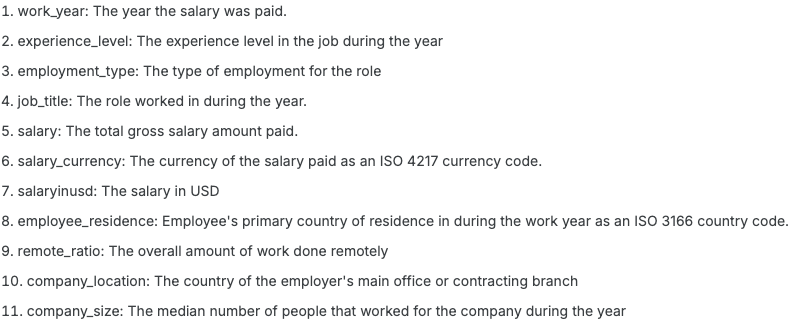
\includegraphics[width=1\linewidth]{graphics/datensatz.png}
    \caption[Beschreibung der Spalten des Datensatzes]{Beschreibung der Spalten des Datensatzes.}
    \label{fig:Datensatz-Kaggle}
\end{figure}

Um den Datensatz weiter anzureichern und die Möglichkeiten der Echtzeitverarbeitung zu demonstrieren, wurde zusätzlich ein Web-Scraper entwickelt. Dieser sammelt Gehaltsdaten von der Webseite Glassdoor unter folgender URL: \url{https://www.glassdoor.de/Job/Data-Scientist-jobs-SRCH_KO0,10.htm} und integriert die gesammelten Informationen direkt in den bestehenden Datensatz. Auf diese Weise werden die Analysen um zusätzliche Aspekte ergänzt, die eine Echtzeitverarbeitung sowie eine erweiterte Visualisierung der Daten ermöglichen. Der Web-Scraper befindet sich im Ordner \lstinline|scraper| und kann durch das Starten des entsprechenden Containers ausgeführt werden.

\newpage

\section{Demonstration von Features}

Die Umsetzung der Lakehouse-Architektur umfasst mehrere Schritte und Features. Zu Beginn wird ein \lstinline|minio|-Container gestartet, der als zentraler Objektspeicher dient. Anschließend erfolgt die Einrichtung durch einen \lstinline|minio-init|-Container. Während dieses Prozesses wird ein Administrator-Konto erstellt, dessen Zugangsdaten aus der \lstinline|.env|-Datei ausgelesen werden. Zudem wird ein Bucket mit dem Namen \lstinline|lakehouse-storage| konfiguriert, der als Speicherort für die verarbeiteten Daten dient.

Abbildung \ref{fig:MinIO-Login} zeigt den Login-Bildschirm von MinIO, der den Zugang zur Verwaltungsoberfläche ermöglicht. 

\begin{figure}[H]
    \centering
    
\includegraphics[width=1\linewidth]{graphics/minio-login.png}
    \caption[MinIO - Login Screen]{MinIO - Login Screen.}
    \label{fig:MinIO-Login}
\end{figure}

Nach erfolgreicher Einrichtung zeigt die MinIO-Oberfläche den konfigurierten Bucket \lstinline|lakehouse-storage|, wie in Abbildung \ref{fig:MinIO-Bucket} dargestellt. Dieser Bucket dient als zentraler Speicherort für Daten im Delta- und Parquet-Format, die im Rahmen der Lakehouse-Architektur verarbeitet und analysiert werden.

\begin{figure}[H]
    \centering
    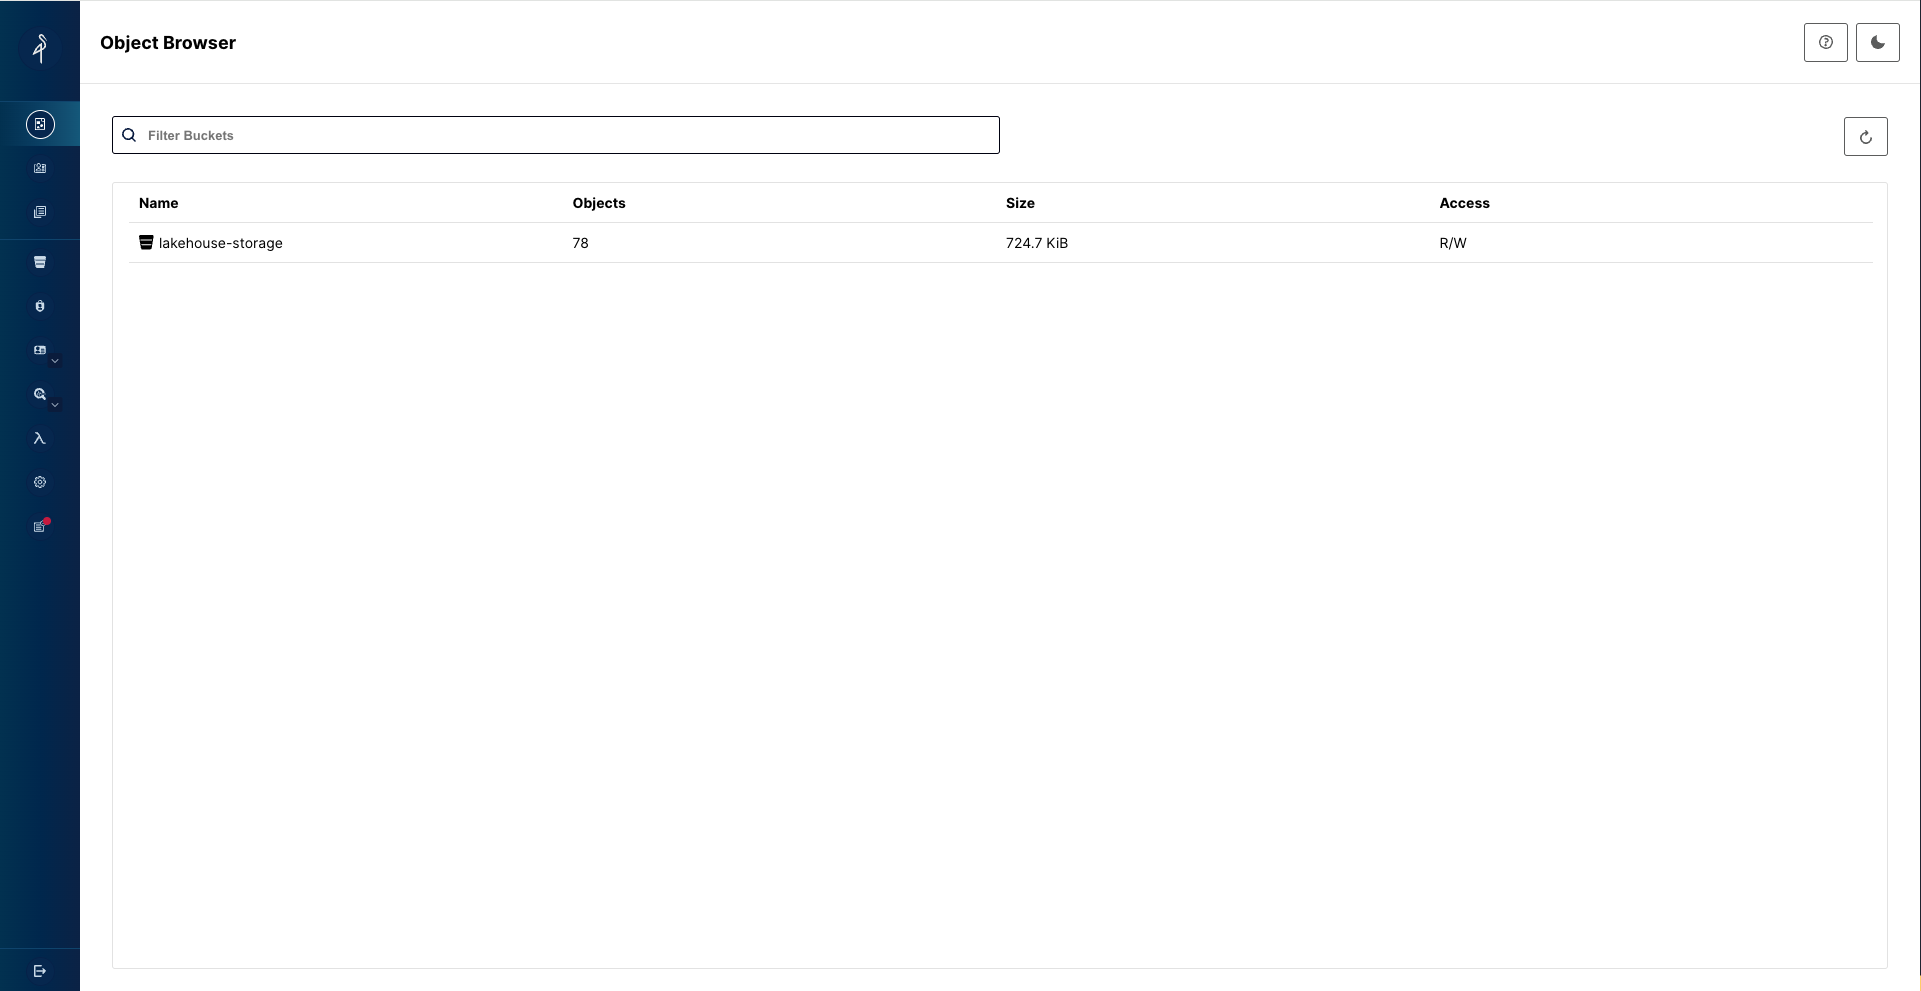
\includegraphics[width=1\linewidth]{graphics/minio.png}
    \caption[MinIO mit erstelltem lakehouse-storage Bucket]{MinIO mit erstelltem \lstinline|lakehouse-storage| Bucket.}
    \label{fig:MinIO-Bucket}
\end{figure}

Anschließend wird ein Spark-Cluster gestartet, bestehend aus einem \lstinline|spark-master|-Container, einem \lstinline|spark-worker|-Container und einem \lstinline|spark-submit|-Container. Dieser Cluster übernimmt die Verarbeitung der Ursprungsdaten aus der Datei \lstinline|ds_salaries.csv|. Dabei werden die Daten in Delta-Tabellen zerlegt und in den MinIO-Speicher hochgeladen, um eine effiziente Speicherung und Weiterverarbeitung zu gewährleisten. Dies markiert den ersten Schritt innerhalb einer Medallion-Architektur, in dem die "Raw" Daten verarbeitet, in Delta-Tabellen überführt und im gemeinsamen Speicher organisiert werden. Gleichzeitig erfolgen erste Transformationen, die die Grundlage für nachfolgende Verarbeitungsschritte bilden. Zudem wird dadurch eine Simulationsumgebung geschaffen, die demonstriert, wie Daten aus verschiedenen Systemen in ein Speicher geladen werden können.

Abbildung \ref{fig:Spark-Cluster} zeigt die Oberfläche des Apache Spark Clusters, die den Status und die laufenden Jobs visualisiert.

\begin{figure}[H]
    \centering
    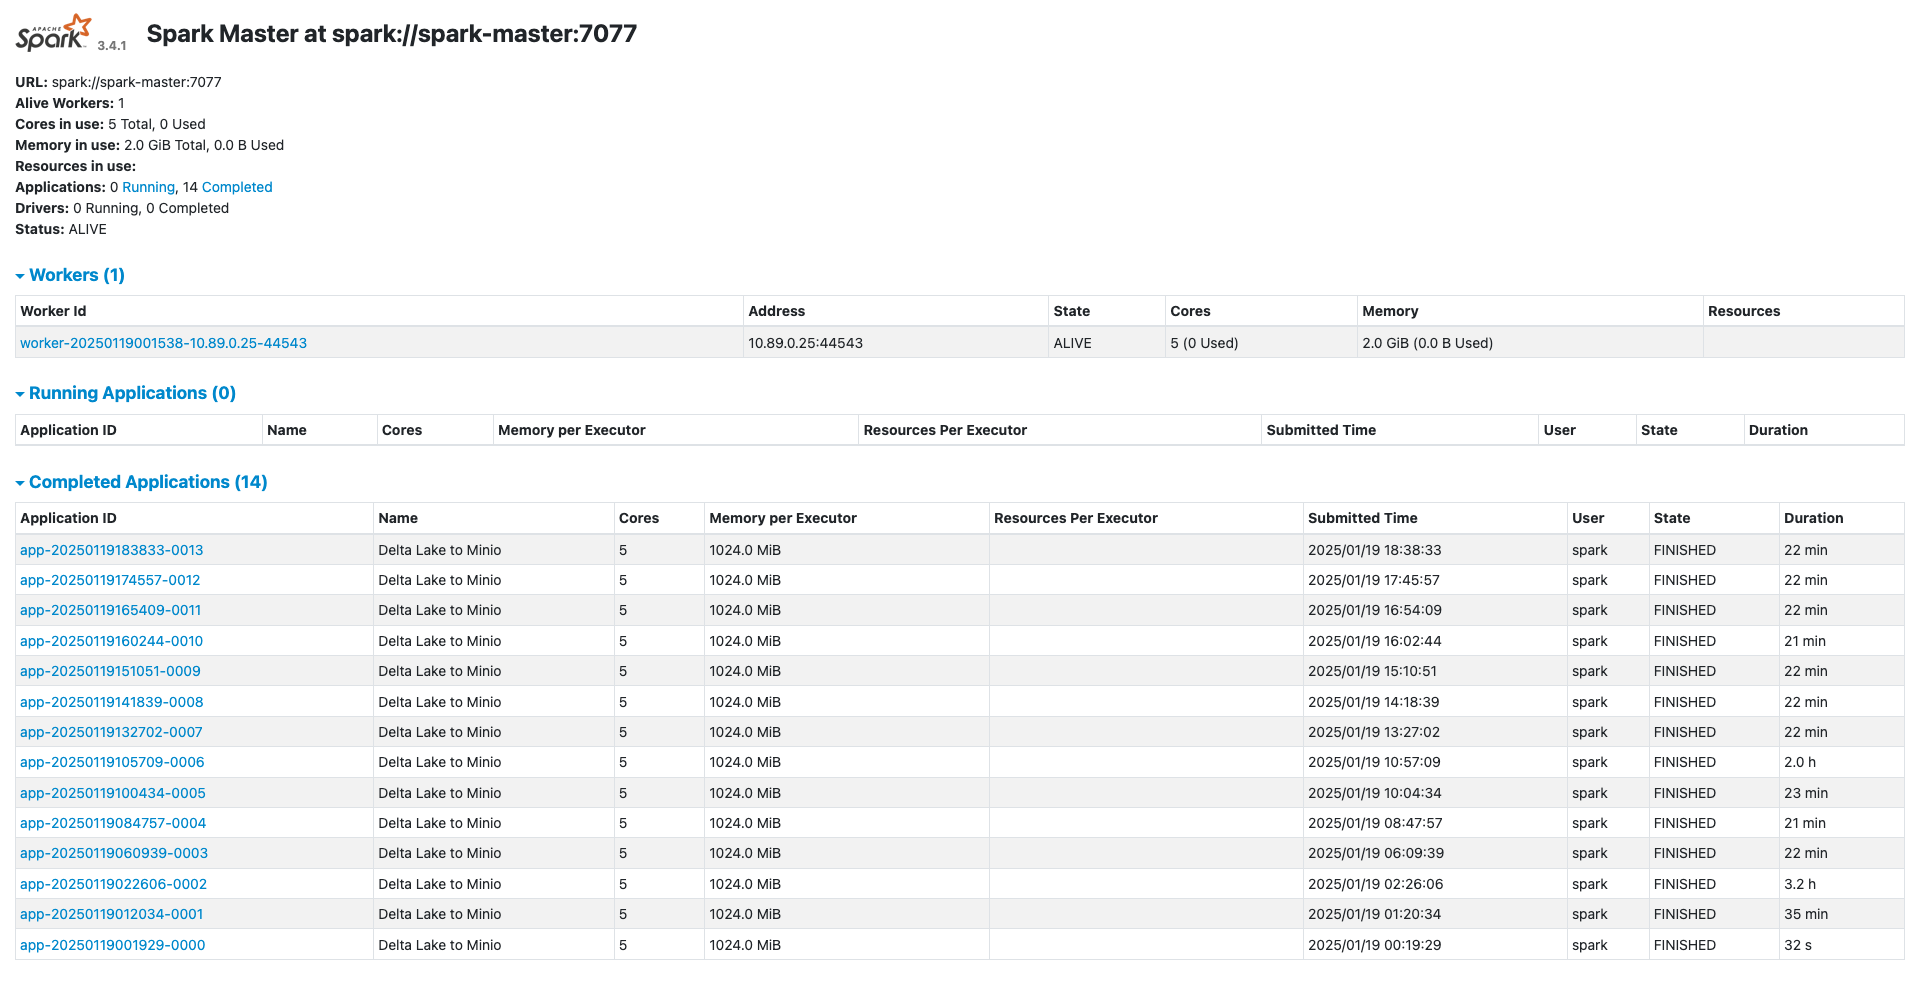
\includegraphics[width=1\linewidth]{graphics/spark.png}
    \caption[Oberfläche des Apache Spark Clusters]{Oberfläche des Apache Spark Clusters.}
    \label{fig:Spark-Cluster}
\end{figure}

Zur Anreicherung des Datensatzes mit zusätzlichen Informationen wird der \lstinline|scraper|-Container eingesetzt. Dieser sammelt Gehaltsdaten von der Webseite Glassdoor, verarbeitet sie mithilfe der Python-Bibliothek \lstinline|pandas| und der Bibliothek \lstinline|Selenium| und fügt sie dem bestehenden Datensatz hinzu (siehe Abbildung \ref{fig:Scraper}). Um eine regelmäßige Aktualisierung der Daten zu gewährleisten, sind sowohl der \lstinline|scraper|-Container als auch der \lstinline|spark-submit|-Container so konfiguriert, dass sie alle 20 Minuten automatisch ausgeführt werden. Dadurch bleibt der MinIO-Speicher stets auf dem neuesten Stand.

\begin{figure}[H]
    \centering
    
\includegraphics[width=0.8\linewidth]{graphics/scraper.png}
    \caption[Ein Ausschnitt einer gescrapten Jobstelle von Glassdoor]{Ein Ausschnitt einer gescrapten Jobstelle von Glassdoor.}
    \label{fig:Scraper}
\end{figure}

Die verarbeiteten Daten werden im MinIO-Speicher in Form von Delta Lake Tabellen gespeichert, wie in Abbildung \ref{fig:Delta-Tables} dargestellt. Diese Tabellen sind in verschiedene logische Partitionen unterteilt, was eine flexible Abfrage und Analyse ermöglicht.

\begin{figure}[H]
    \centering
    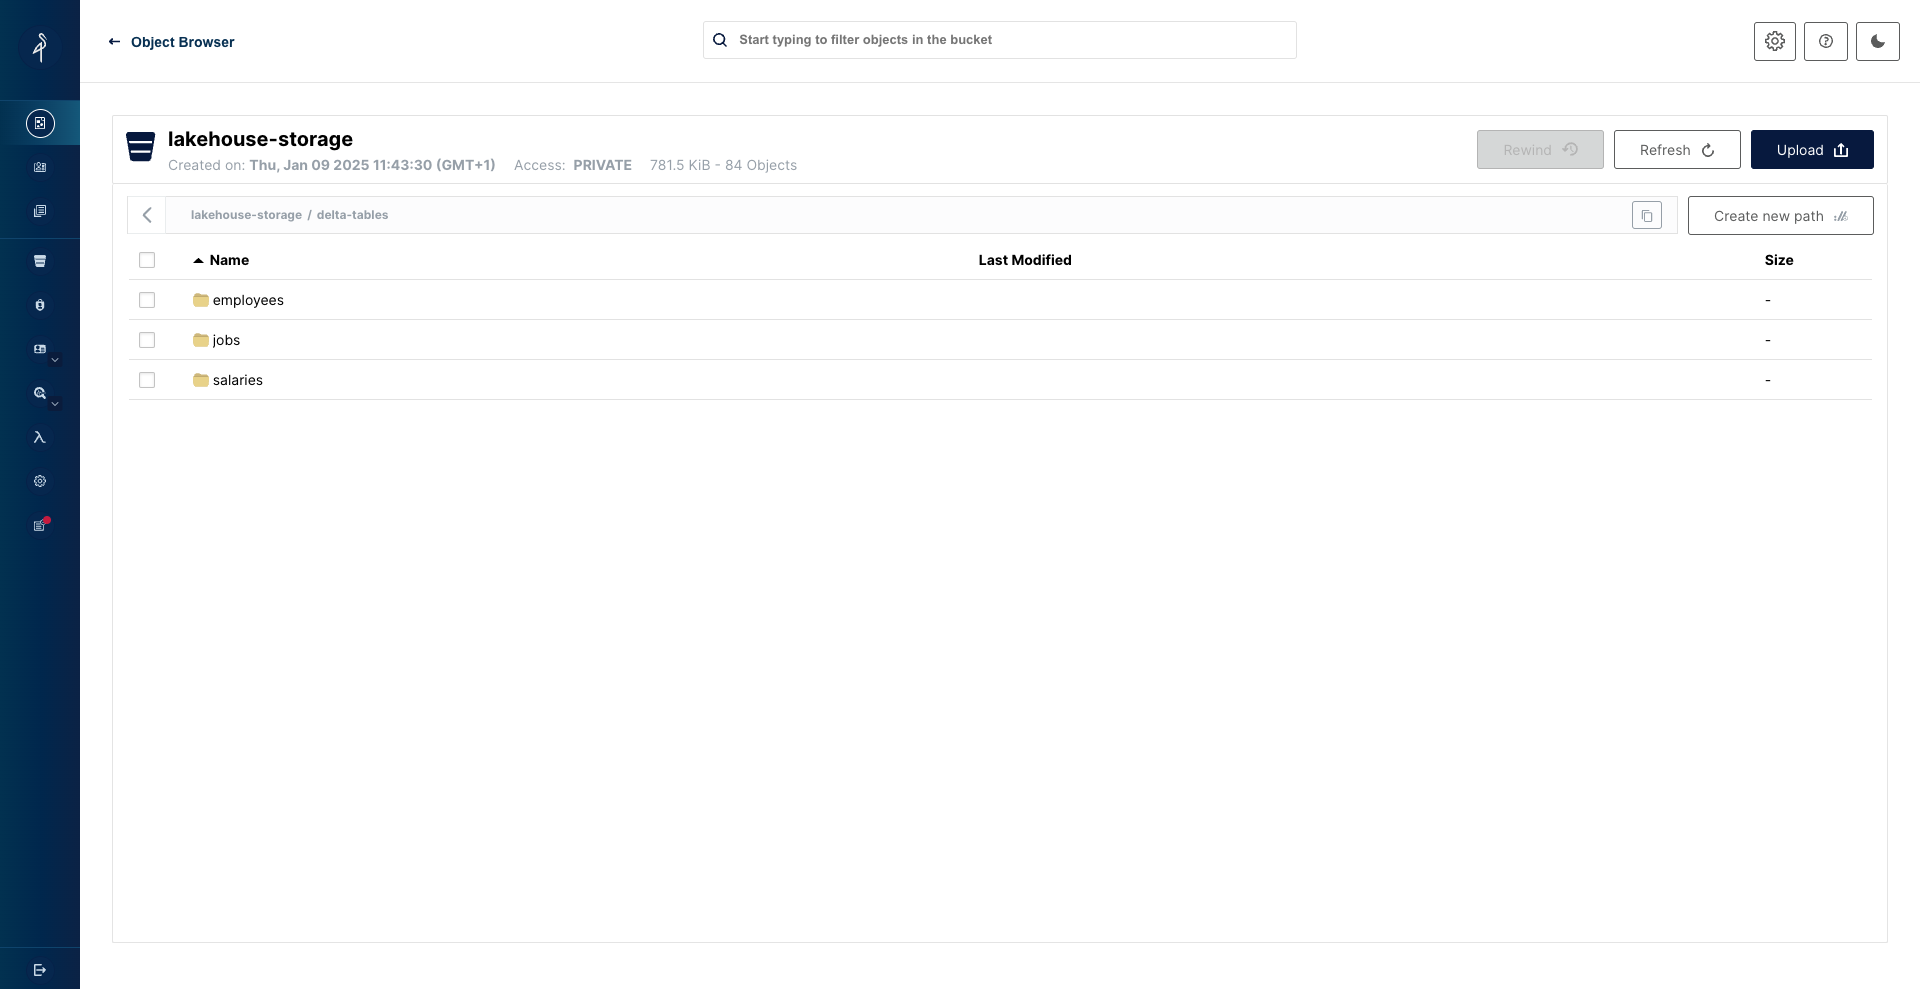
\includegraphics[width=1\linewidth]{graphics/delta-folder.png}
    \caption[Zerlegte CSV-Datei in Delta Lake Tabellen]{Zerlegte CSV-Datei in Delta Lake Tabellen.}
    \label{fig:Delta-Tables}
\end{figure}

Eine detaillierte Ansicht der gespeicherten Daten zeigt die Employee-Tabelle, die aus mehreren Parquet-Dateien besteht. Diese Dateien ermöglichen eine effiziente Speicherung und Bereitstellung großer Datenmengen, wie in Abbildung \ref{fig:Delta-Employee-Table} illustriert.

\begin{figure}[H]
    \centering
    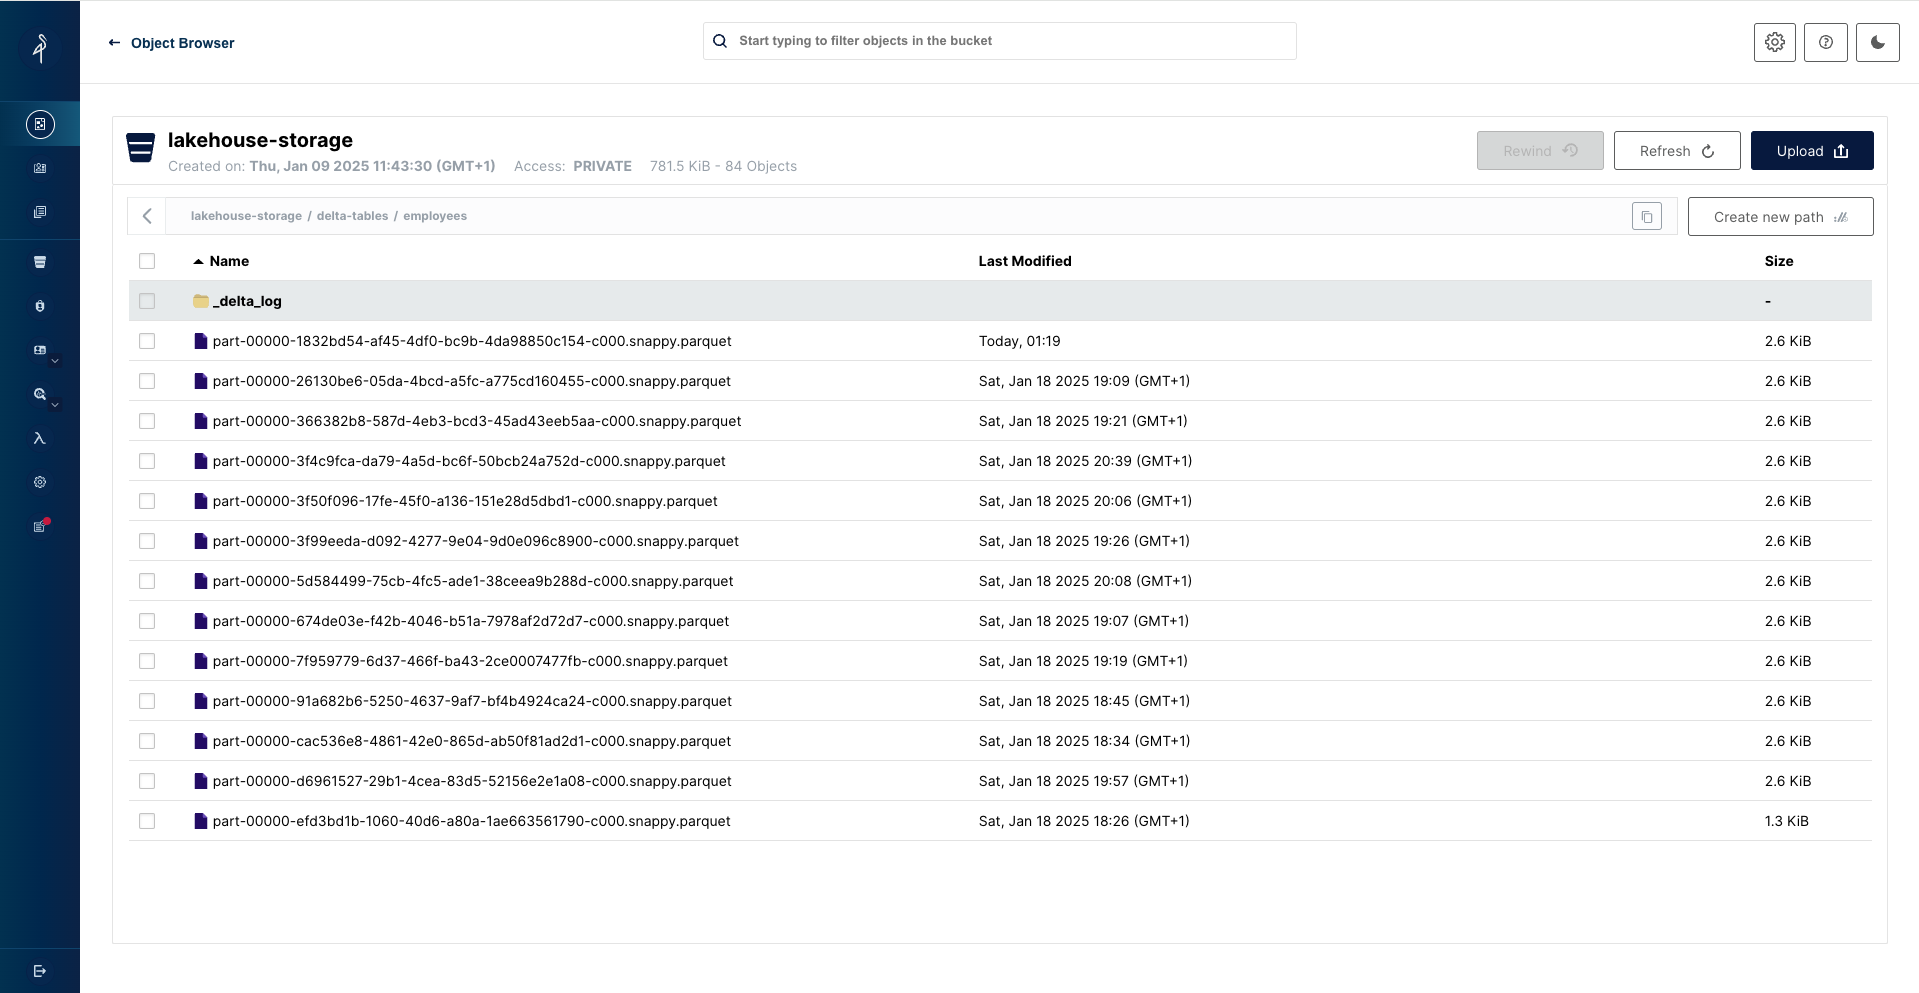
\includegraphics[width=1\linewidth]{graphics/delta-folder-employees.png}
    \caption[Delta Lake Employee Tabelle mit Parquet-Dateien]{Delta Lake Employee Tabelle mit Parquet-Dateien.}
    \label{fig:Delta-Employee-Table}
\end{figure}

Die drei Delta-Tabellen werden von DuckDB eingelesen und anschließend mit Ibis zusammengeführt, verarbeitet und analysiert. Die dabei erstellten Analysen bieten wertvolle Einblicke für geschäftliche Anwendungen und repräsentieren das Gold-Layer der Medallion-Architektur. 

\begin{figure}[H]
    \centering
    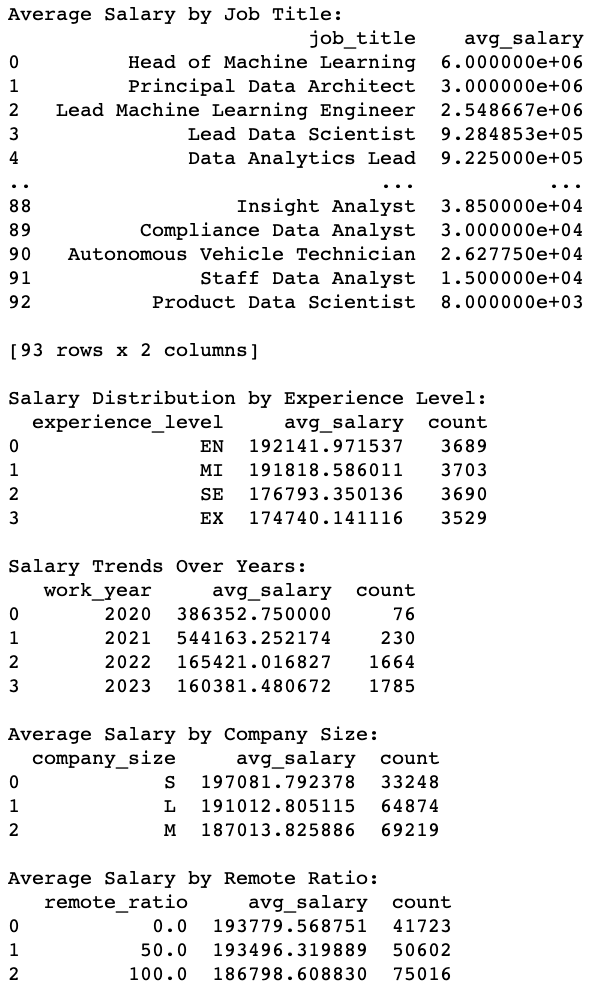
\includegraphics[width=0.5\linewidth]{graphics/analysen.png}
    \caption[Analysen mittels DuckDB und Ibis zur Visualisierung in Apache Superset]{Analysen mittels DuckDB und Ibis zur Visualisierung in Apache Superset.}
    \label{fig:Delta-Employee-Table}
\end{figure}

Die Visualisierung der Analyseergebnisse wird in Apache Superset realisiert, wo Dashboards und Diagramme erstellt werden, um detaillierte Einblicke in Gehaltsstrukturen und Arbeitsbedingungen zu bieten. Dieser Schritt bildet den Abschluss der Medallion-Architektur und demonstriert die vollständige Umsetzung einer Lakehouse-Architektur.

Aus den erstellten Charts und Dashboards lassen sich wertvolle Erkenntnisse ableiten, die eine fundierte Grundlage für strategische Entscheidungen bieten. 
Das erste Diagramm (Abbildung \ref{fig:chart1}) zeigt die durchschnittlichen Gehälter nach Jobtiteln und verdeutlicht, welche Rollen innerhalb des Bereichs Data Science am höchsten vergütet werden. Diese Analyse kann dazu genutzt werden, strategische Personalentscheidungen zu treffen oder Gehaltspakete wettbewerbsfähig zu gestalten.

\begin{figure}[H]
    \centering
    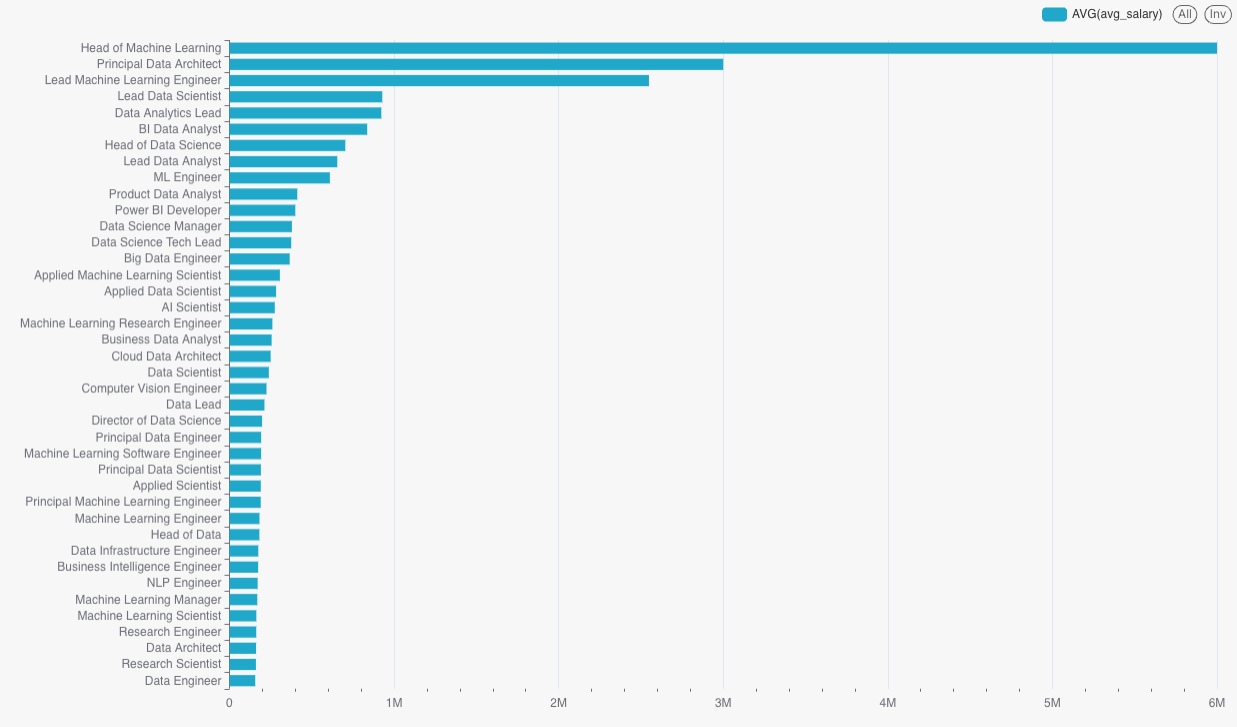
\includegraphics[width=1\linewidth]{graphics/salary-by-job.jpg}
    \caption[Durchschnittsgehälter nach Jobpositionen]{Durchschnittsgehälter nach Jobpositionen.}
    \label{fig:chart1}
\end{figure}

Das zweite Diagramm (Abbildung \ref{fig:Salary-over-years}) zeigt die Gehaltsentwicklung über die Jahre. Es wird ersichtlich, wie sich die durchschnittlichen Gehälter im Zeitverlauf verändert haben. Besonders auffällig ist der Höhepunkt im Jahr 2021, gefolgt von einem deutlichen Rückgang in den darauffolgenden Jahren, dies könnte jedoch auch auf fehlende Daten in diesem Jahr zurückzuführen sein. 

\begin{figure}[H]
    \centering
    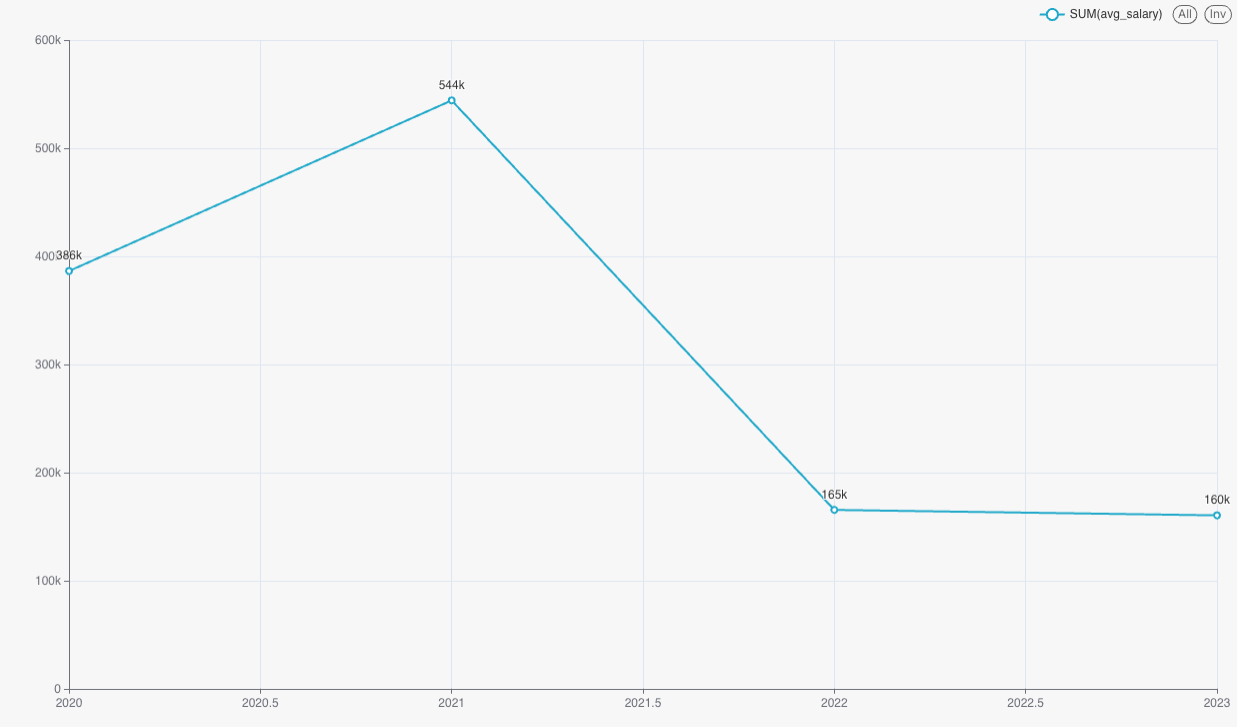
\includegraphics[width=0.8\linewidth]{graphics/salary-trend-year.jpg}
    \caption[Durchschnittliche Gehaltsentwicklung bei Data Science Jobs über die Jahre]{Durchschnittliche Gehaltsentwicklung bei Data Science Jobs über die Jahre.}
    \label{fig:Salary-over-years}
  \end{figure}

\newpage  

Im Anhang sind drei weitere Diagramme aus den Analysen mit DuckDB, Ibis und Apache Superset dargestellt (siehe Anhang \ref{anhang:zusaetlichediagramme}). Diese Visualisierungen verdeutlichen die Vielseitigkeit und den Mehrwert der in der Lakehouse-Architektur implementierten Datenanalyse.

Abschließend bleibt anzumerken, dass die Konfiguration von Apache Superset den einzigen manuellen Schritt innerhalb der Umsetzung darstellt. Dabei müssen Datenquellen und Dashboards eingerichtet werden, um benutzerspezifische Visualisierungen zu ermöglichen. Während dieses Prozesses trat ein nicht behebbarer Fehler auf. Das Hinzufügen von Charts zu einem Dashboard führte wiederholt zu einem Core Dump, siehe Anhang \ref{anhang:apachesuperset}. Weder die Log-Analyse noch Tests auf unterschiedlichen Endgeräten konnten das Problem lösen, was auf einen möglichen Fehler in Apache Superset hinweist. Dennoch konnte die Funktionalität der Lakehouse-Architektur erfolgreich demonstriert werden, da die Visualisierung der Daten weiterhin über die Erstellung von Charts möglich war.



%%% Ende des eigentlichen Inhalts %%%


%%% Quellenverzeichnisse (keine Anpassung nötig) %%%
\clearpage
\literaturverzeichnis
%%% Ende Quellenverzeichnisse %%%


%%% Erklärung (keine Anpassungen nötig) %%%
% steht ganz am Ende des Dokuments
\cleardoublepage
\clearpage

\thispagestyle{empty}
\DEoEN{%
{\LARGE\textsf{\textbf{Erklärung zur Verwendung generativer KI-Systeme}}\bigskip}

Bei der Erstellung der eingereichten Arbeit habe ich die nachfolgend aufgeführten auf künstlicher Intelligenz (KI) basierten Systeme benutzt:

\begin{enumerate}
\item Consensus
\item ChatGPT-4o
\end{enumerate}

Ich erkläre, dass ich

\begin{itemize}
  \item mich aktiv über die Leistungsfähigkeit und Beschränkungen der oben genannten 
KI-Systeme informiert habe,\footnote{U.a. gilt es hierbei zu beachten, dass an KI weitergegebene Inhalte ggf. als Trainingsdaten genutzt und wiederverwendet werden. Dies ist insb. für betriebliche Aspekte als kritisch einzustufen.}
  \item die aus den oben angegebenen KI-Systemen direkt oder sinngemäß übernommenen Passagen gekennzeichnet habe,
%
% In der Fußnote Ihrer Arbeit geben Sie die KI als Quelle an, z.B.: 
% Erzeugt durch Microsoft Copilot am dd.mm.yyyy. 
% Oder: Entnommen aus einem Dialog mit Perplexity vom dd.mm.yyyy. 
% Oder: Absatz 2.3 wurde durch ChatGPT sprachlich geglättet.
%
  \item überprüft habe, dass die mithilfe der oben genannten KI-Systeme generierten und von mir übernommenen Inhalte faktisch richtig sind,
  \item mir bewusst bin, dass ich als Autorin bzw. Autor dieser Arbeit die Verantwortung für die in ihr gemachten Angaben und Aussagen trage.
\end{itemize}

Die oben genannten KI-Systeme habe ich wie im Folgenden dargestellt eingesetzt: 


\begin{tabular}{|p{4cm}|p{3cm}|p{7cm}|}
  \hline
  \textbf{Arbeitsschritt in der wissenschaftlichen Arbeit} & 
  \textbf{Eingesetzte(s) KI-System(e)} & 
  \textbf{Beschreibung der Verwendungsweise} \\
  \hline
  Literaturrecherche & 
  Consensus & 
  Unterstützung bei der Suche nach wissenschaftlicher Literatur. \\
  \hline
  Korrektur der Arbeit & 
  ChatGPT-4 & 
  Einzelne Kapitel der Arbeit wurden ChatGPT zum Korrigieren gegeben. \\
  \hline
  Fehleranalyse von Programmcode & 
  ChatGPT-4 & 
  Einige Programmzeilen wurden an ChatGPT übergeben, um sie auf Fehler zu prüfen. \\
  \hline
\end{tabular}
} % Ende deutscher Teil
{% Beginn englische Erklaerung
{\LARGE\textsf{\textbf{Declaration on the Use of Generative AI Systems}}\bigskip}

In preparing the submitted work, I have used the following artificial intelligence (AI)-based systems:

\begin{enumerate}
\item
\item
\item \ldots
\end{enumerate}

I hereby declare that I

\begin{itemize}
  \item actively informed myself about the capabilities and limitations of the above-mentioned AI systems,\footnote{In particular, it should be noted that content passed on to AI may be used as training data and reused. This is to be considered critical, especially for operational aspects.}
  \item indicated passages directly or indirectly adopted from the above-mentioned AI systems,
%
% In the footnote of your work, cite the AI as the source, e.g.:
% Generated by Microsoft Copilot on mm.dd.yyyy. 
% Or: Taken from a dialogue with Perplexity on mm.dd.yyyy. 
% Or: Paragraph 2.3 was linguistically smoothed by ChatGPT.
%
  \item verified that the content generated and adopted by me using the above-mentioned AI systems is factually correct,
  \item am aware that as the author of this work, I bear responsibility for the statements and information provided in it.
\end{itemize}

I have utilized the above-mentioned AI systems as illustrated below: 

\begin{center}
\begin{tabular}{|p{4cm}|p{3cm}|p{7cm}|}
    \hline
    \textbf{Task in the scientific work} &
%
% Examples of such tasks include: idea generation, 
% conception of the work, literature search, literature analysis, 
% literature management, selection of methods, data collection, 
% data analysis, generation of program code
%
% If you are unsure whether you need to specify an AI system used, 
% consult your supervisor.
%
	 \textbf{AI System(s) Used} & \textbf{Description of Usage} \\
    \hline
    & & \\ % Placeholder for your entries, insert your information here
    \hline
    & & \\ % (Expand the table as needed and continue on subsequent pages)
    \hline
    & & \\
    \hline
    & & \\
    \hline
  \end{tabular}
\end{center}
}

\clearpage

\thispagestyle{empty}

{\LARGE\textsf{\textbf{\DEoEN{Erklärung}{Declaration}}}\bigskip}

% \typMeinerArbeit und \themaMeinerArbeit werden in config.tex definiert
\DEoEN{%
Ich versichere hiermit, dass ich die vorliegende Arbeit mit dem Thema: \emph{Open Source Lakehouse Container (mittels DuckDB)} selbstständig verfasst und keine anderen als die angegebenen Quellen und Hilfsmittel benutzt habe.
Ich versichere zudem, dass die eingereichte elektronische Fassung mit der gedruckten Fassung übereinstimmt.%
}{%
I hereby insure that I have personally authored this thesis with the topic: \emph{\themaMeinerArbeit} and have used no sources and aids other than those indicated. I also insure that the submitted electronic version corresponds to the printed version.%
}

\vspace{3cm}

\begin{center}
\begin{tabular}{ccc}
Stuttgart, \abgabeDatum & \hspace{0.3\linewidth} & 
\includegraphics[width=0.3\linewidth]{graphics/signature.png}\\
(\DEoEN{Ort, Datum}{place, date}) & \hspace{0.3\linewidth} & (\DEoEN{Unterschrift}{signature})
\end{tabular}
\end{center}


\end{document}